% ~ 6 pages
\chapter{Theoretical Background}
\label{sec:theory}

In this chapter the theoretical background for the studies in this thesis is
provided. First the Standard Model of particle physics is introduced and its
problems discussed. Then the physics of tau leptons is discussed with a focus on
hadronic decays of the tau lepton.

\section{The Standard Model of Particle Physics}

The Standard Model of particle physics describes the current understanding of
elementary particles and interactions between them. The Standard Model has been
extensively tested since its origin and shows a good agreement with experimental
results. However, it does not offer a full description of particle physics as it
does not explain interactions of massive particles via gravity.

In Figure~\ref{fig:sm_particles} the elementary particles of the Standard Model
are shown. They can be divided into the fermions consisting of particles with
spin-half and bosons with integer spin. In 2012 the ATLAS and CMS experiments at
the Large Hadron Collider (LHC) discovered a new scalar boson with a mass
of~$m_\text{h} \approx \SI{125}{\GeV}$~\cite{higgs_atlas, higgs_cms}, which is
consistent with the Higgs boson predicted by the Standard Model.

\begin{figure}[htb]
  \centering
  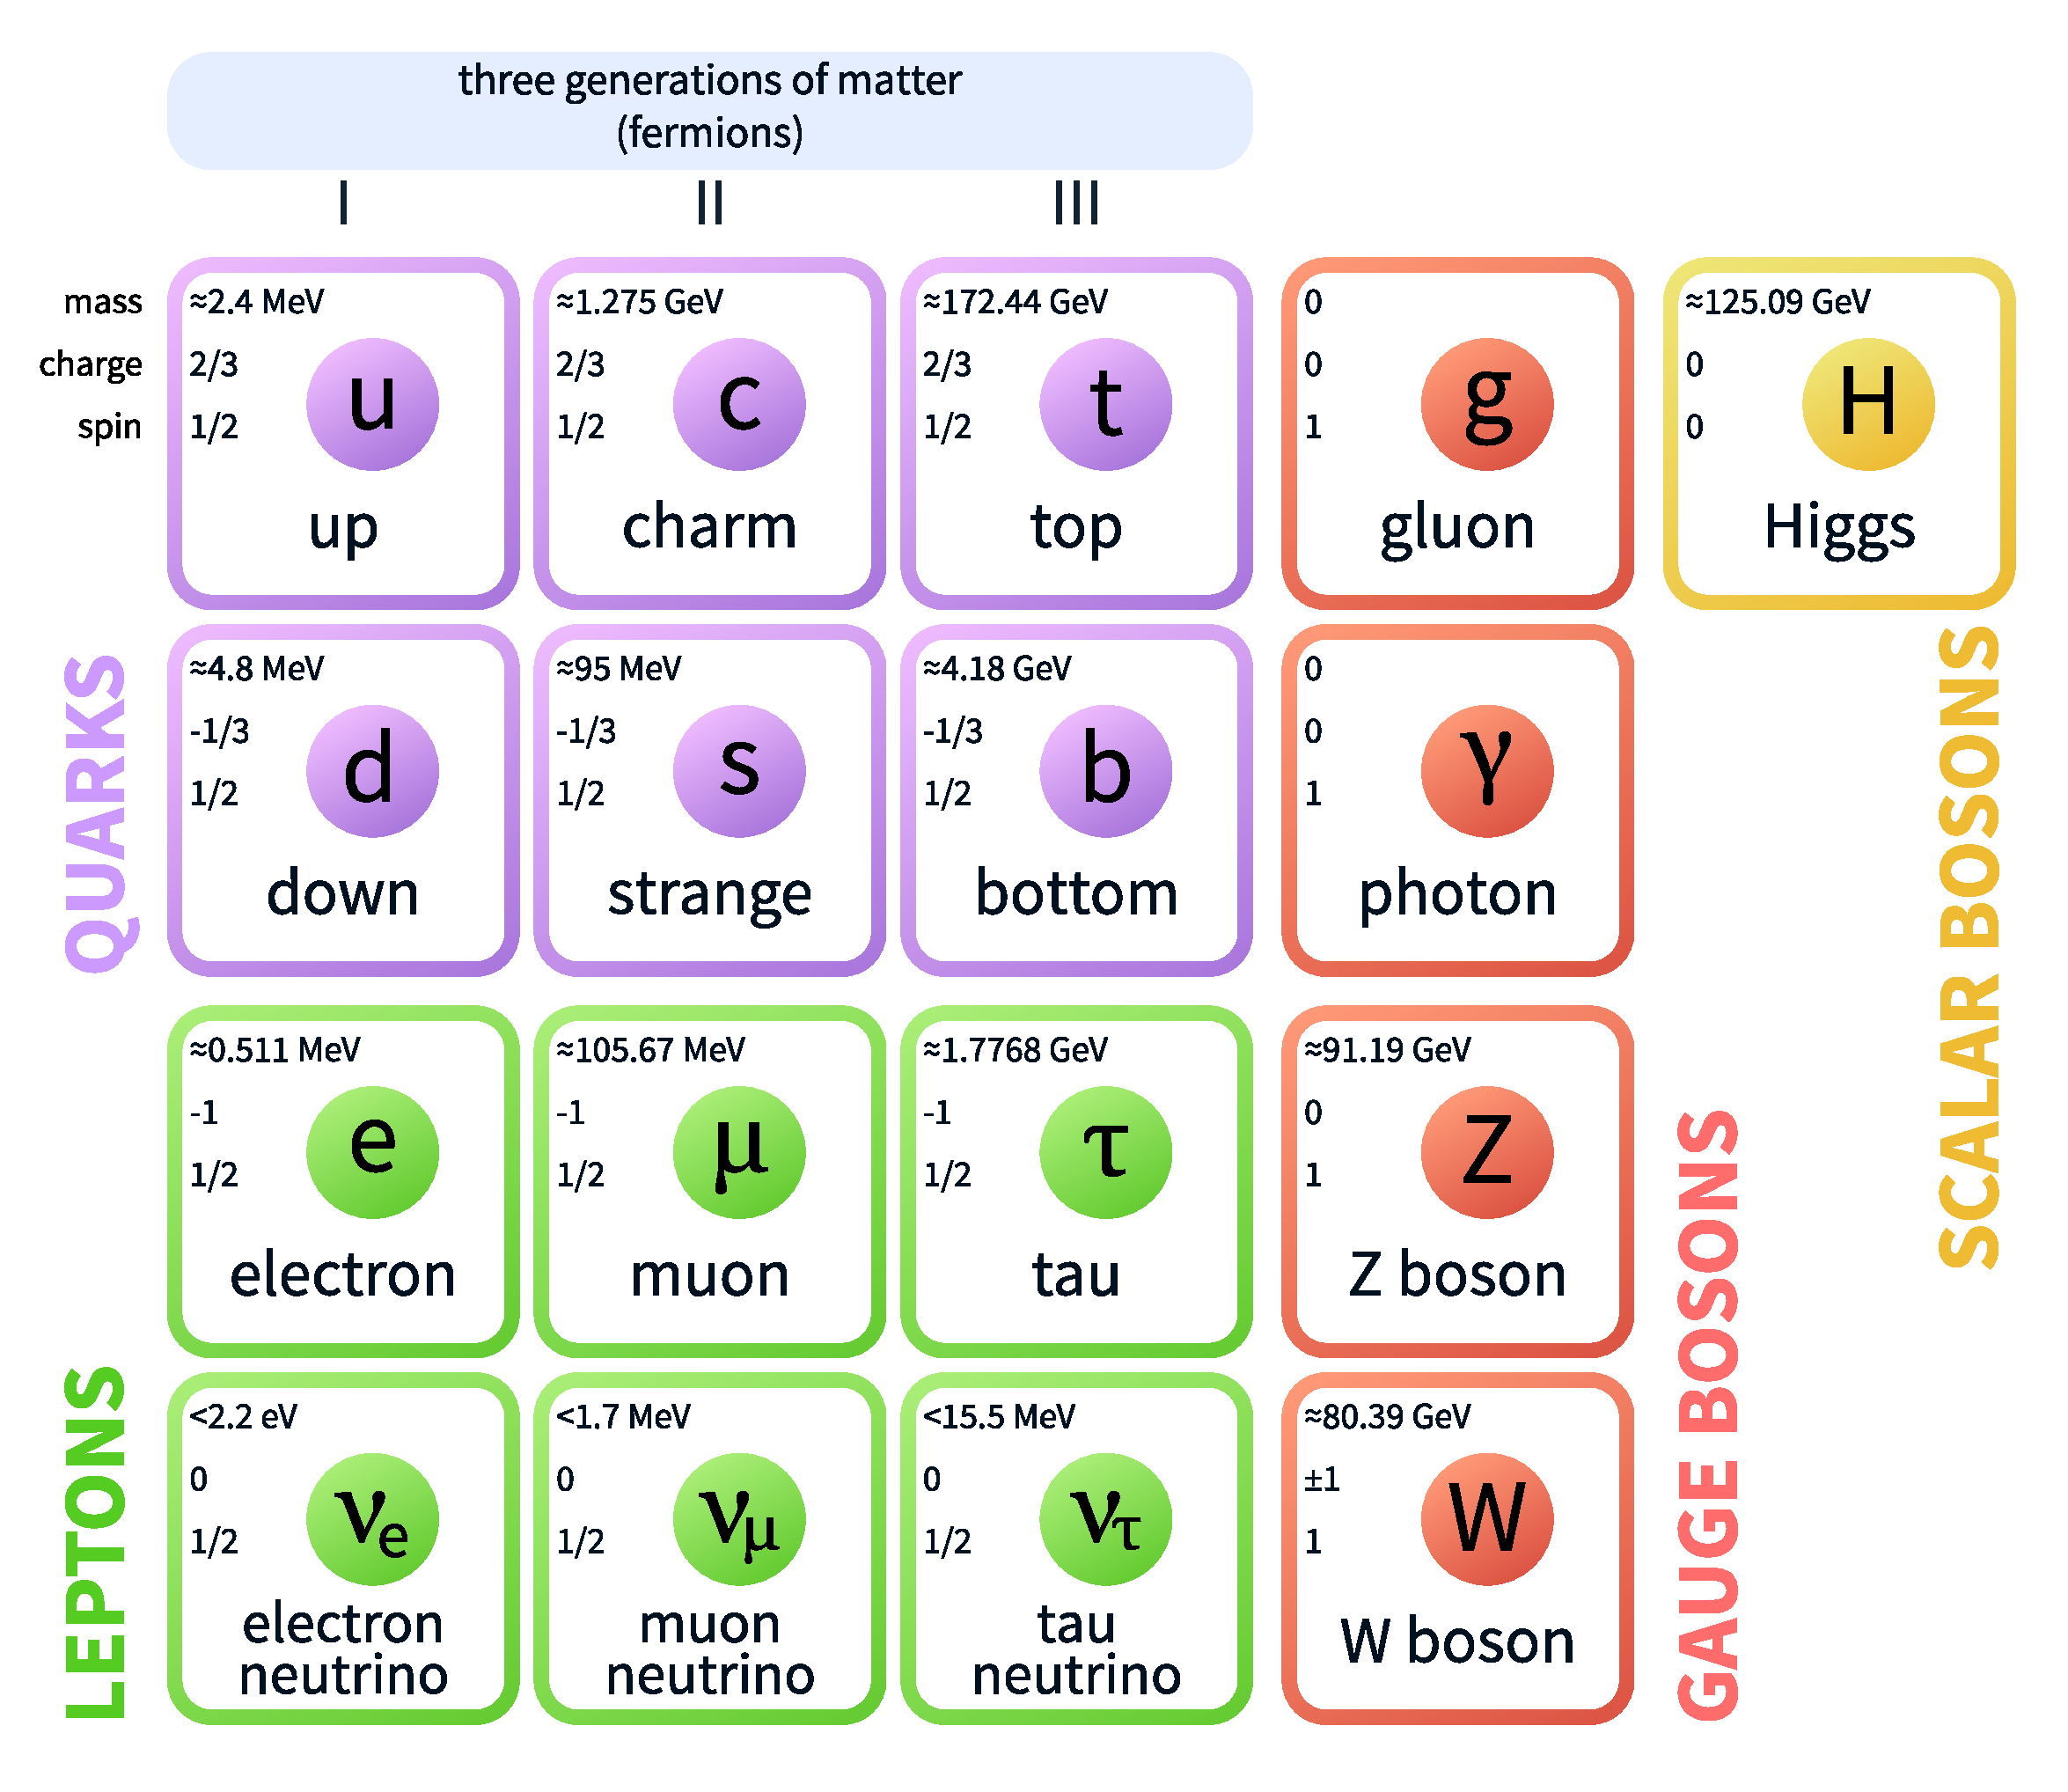
\includegraphics[width=0.7\textwidth]{./figures/theory/sm_particles.pdf}
  \caption{Particles of the Standard Model. Image modified from
    Ref.~\cite{sm_wiki}.}
  \label{fig:sm_particles}
\end{figure}

In the following the elementary particles and their interactions are described.
The fermions of the Standard Model form the known matter in the Universe. Their
dynamics are described by the Dirac equation, while interactions between them
are mediated by spin-1 gauge bosons. The nature of these interactions is
described by quantum field theories and the local gauge principle. The fermions
are divided into up- and down-type quarks with a charge of~$2/3$ and~$-1/3$,
respectively and leptons consisting of the charged leptons and the neutrinos.
Additionally, the fermions are divided into three generations with identical
properties with the exception of the increasing particle mass with each
generation. The first generation consisting of the electron, electron neutrino,
up- and down-quark makes up the stable matter in the Universe. The fermions of
the second and third generation are only produced in high-energy particle
collisions. Each fermion has a corresponding antiparticle with the same mass but
with inverted additive quantum numbers including the electric charge.

The strong interaction between quarks is described by quantum chromodynamics.
The exchange particle of the strong force is the massless gluon, which couples
to the so called color charge. The quarks as well as the gluons carry color
charge allowing $qqg$-vertices as well as gluon self-coupling in triple and
quartic gluon vertices. Experimentally, free quarks are not observed but only
color-neutral bound states called hadrons. This is known as colour confinement
and leads to the formation of collimated jets of hadrons in processes creating
high-energy quarks or gluons.\todo{Ben -- write sth.\ about the hadronisation
  process. Parton shower -- perturbative QCD, Hadronisation -- nonperturbative
  QCD}

The electromagnetic interaction between particles carrying electric charge is
described by quantum electrodynamics. The mediating gauge boson is the massless
photon, which couples to electrically charged particles including quarks,
charged leptons and the $W^\pm$~boson.

The weak interaction is mediated by the massive $Z$ and $W^\pm$~bosons, which
couple to the weak charges carried by all fermions. Additionally, couplings
between the weak bosons itself are allowed. The weak charged-current interaction
is mediated by the $W^\pm$~boson and couples to chiral left-handed particles and
chiral right-handed antiparticles, thereby maximally violating $\text{P}$
symmetry. The weak charged-current allows flavour changes in the quark sector.
In contrast to this, the weak neutral-current interaction mediated by the
$Z$~boson does not allow flavour changes. The $Z$ couples to both left- and
right-handed particles although with different strength. The weak interaction is
observed to violate \cp symmetry in the quark
sector~\cite{cp_violation_quark_sector, cp_violation_quark_sector_2}, while \cp
violation the the lepton sector is not yet confirmed.

The electromagnetic and weak interactions are unified in the electroweak theory
developed by Glashow, Salam and Weinberg~\cite{glashow, salam, weinberg}. The
local gauge symmetry~$\mathrm{SU}(2)_\text{L}$ generating the weak
charged-current interaction and the $W^+$, $W^-$ boson fields as well as a
neutral field $W^{(3)}$ coupling to chiral left-handed particles. The
electroweak unification introduces a $\mathrm{U}(1)_Y$ gauge symmetry,
where~$Y = 2 (Q - T_3)$ is the weak hypercharge with the electric charge~$Q$ and
the third component of the weak isospin~$T_3$. The~$\mathrm{U}(1)_Y$ symmetry
generates a neutral field~$B$ that mixes with~$W^{(3)}$ giving rise to the
photon and $Z$ boson fields~\cite{thomson}, thus combining the weak and the
electromagnetic interaction.

The non-vanishing masses of the $W^\pm$ and $Z$ bosons break the local gauge
invariance of the electroweak theory when introducing a mass term into the
Lagrangian. To maintain the gauge principle a different approach called the
Higgs mechanism~\cite{englert_brout, higgs} is introduced such that the gauge
bosons of the weak interaction can acquire their mass in a process called
spontaneous symmetry breaking. For this a doublet of complex scalar fields with
non-vanishing vacuum expectation value is introduced. This breaks the symmetry
of the Lagrangian and introduces four degrees of freedom. Three are absorbed
into the $W^+$, $W^-$ and $Z$ bosons giving them mass. The remaining neutral and
scalar component becomes the physical Higgs boson~\cite{thomson}. The Higgs
mechanism is also used to generate masses of the fermions, however neutrinos are
assumed to be massless in the Standard Model. The coupling of the Higgs boson to
fermions is called Yukawa coupling and its strength is proportional to the mass
of the fermion~\cite{thomson}.

\subsection{Problems of the Standard Model}

The Standard Model predicts and has been extensively tested. However, some
phenomena remain unexplained in the Standard Model:
\begin{description}
\item[Gravity] Currently, no complete and consistent quantum field theory of
  gravity exists. Therefore, the Standard Model cannot describe the
  gravitational interaction between massive particles.

\item[Dark matter] The Standard Model does not provide a weakly interacting
  massive particle that explains both the observed gravitational interaction of
  dark matter as well as the large-scale structure of the observable Universe.

\item[Origin of neutrino masses] The discovery of neutrino
  oscillations~\cite{superk_neutrino, sno_neutrino_1, sno_neutrino_2} show that
  neutrinos have mass. The origin of this mass is not determined in the Standard
  Model. It can be generated using the Higgs mechanism making neutrinos Dirac
  particles. Another possibility is neutrinos being Majorana particles, in which
  case the seesaw mechanism could explain the experimentally observed mass scale
  of neutrinos.

\item[Matter--antimatter asymmetry] The baryon number and $\mathcal{CP}$
  violation required by the Sakharov conditions~\cite{sakharov} to explain the
  observed matter--antimatter asymmetry, cannot be provided in the Standard
  Model.

\item[Hierarchy problem] The Higgs boson mass is modified by radiative
  corrections due to fermionic and bosonic loops in the Higgs
  propagator~\cite{bettini}. At high energy scales the Higgs mass would be
  large, requiring fine-tuning of the contributions to the Higgs mass to keep it
  at the electroweak scale~\cite{thomson}. Supersymmetry offers a solution to
  this problem, cancelling the corrections.

\item[Unification of the forces] The couplings of the three interactions
  described in the Standard Model are of the same order of magnitude at the
  electoweak energy scale. They might converge at even higher energies,
  suggesting that the Standard Model is only a low-energy manifestation of a
  unified theory~\cite{thomson}.

\item[Number of parameters] A total of 26 free parameters consisting of 12
  fermion masses, 3 coupling constants, the vacuum expectation value of the
  Higgs field and mass of the Higgs boson, 6 mixing angles and 2 phases in the
  PMNS and CKM matrix and potentially a $\mathcal{CP}$~violating phase of the
  strong interaction, are needed to describe the Standard Model~\cite{thomson}.
  The large number of parameters is sometimes viewed as inelegant for describing
  a fundamental theory.
\end{description}
Explanations for these issues need to extend the Standard Model or introduce new
theories like Supersymmetry or Grand Unified Theories.

\section{Tau Leptons}

The tau lepton was discovered in 1975 by Martin Lewis Perl \textit{et al.} with
the LBL detector at the SPEAR electron--position collider at SLAC~\cite{perl}.
With a mass of~\SI{1776.86 +- 0.12}{\MeV} it is the heaviest lepton in the
Standard Model and has a proper lifetime of \SI{290.3 +-
  0.5}{\femto\second}~\cite{pdg}.

\subsection{Decay of the Tau Lepton}

The tau lepton decays via the weak charged-current interaction shown in
Figure~\ref{fig:tau_feynman}. It is more than twelve times heaver than pions and
is therefore the only known lepton in the Standard Model that can decay
leptonically and hadronically. The main decay modes of the tau lepton are
summarised in Figure~\ref{fig:tau_branching_ratios}. The leptonic
modes~\mbox{$\tau^- \to e^- \bar{\nu}_e \nu_\tau$}
and~\mbox{$\tau^- \to \mu^- \bar{\nu}_\mu \nu_\tau$} make up approximately
\SI{35}{\percent} of tau decays, with almost equal branching fractions
to~$e^- \bar{\nu}_e \nu_\tau$ and~$\mu^- \bar{\nu}_\mu \nu_\tau$ due to lepton
universality. The majority of tau decays proceed via hadronic decay modes
producing charged and neutral mesons along with a tau neutrino. The production
of strange quarks is suppressed by a factor
of~$|V_{us}|^2 / |V_{ud}|^2 \approx 1/18$ with elements~$V$ of the CKM matrix
and neglecting any phase space differences. As a result the final state after
hadronisation typically consists of charged and neutral pions, while kaons are
rarely produced. Due to the unit charge of the tau lepton, the decay products of
a tau lepton always contain an odd number of charged particles. Tau decays with
$n$ charged daughter particles are called $n$-prong decays. With a branching
fraction of more than \SI{99}{\percent}, the vast majority of taus decays are 1-
or 3-prong~\cite{pdg}. \todo{intermediate meson resonances? $h^- \pi^0 \nu_\tau$
  -- $\rho(770)$, Modes with 3 pions $a_1(1260)$}

\begin{figure}[htb]
  \begin{subfigure}[b]{0.47\textwidth}
    \centering
    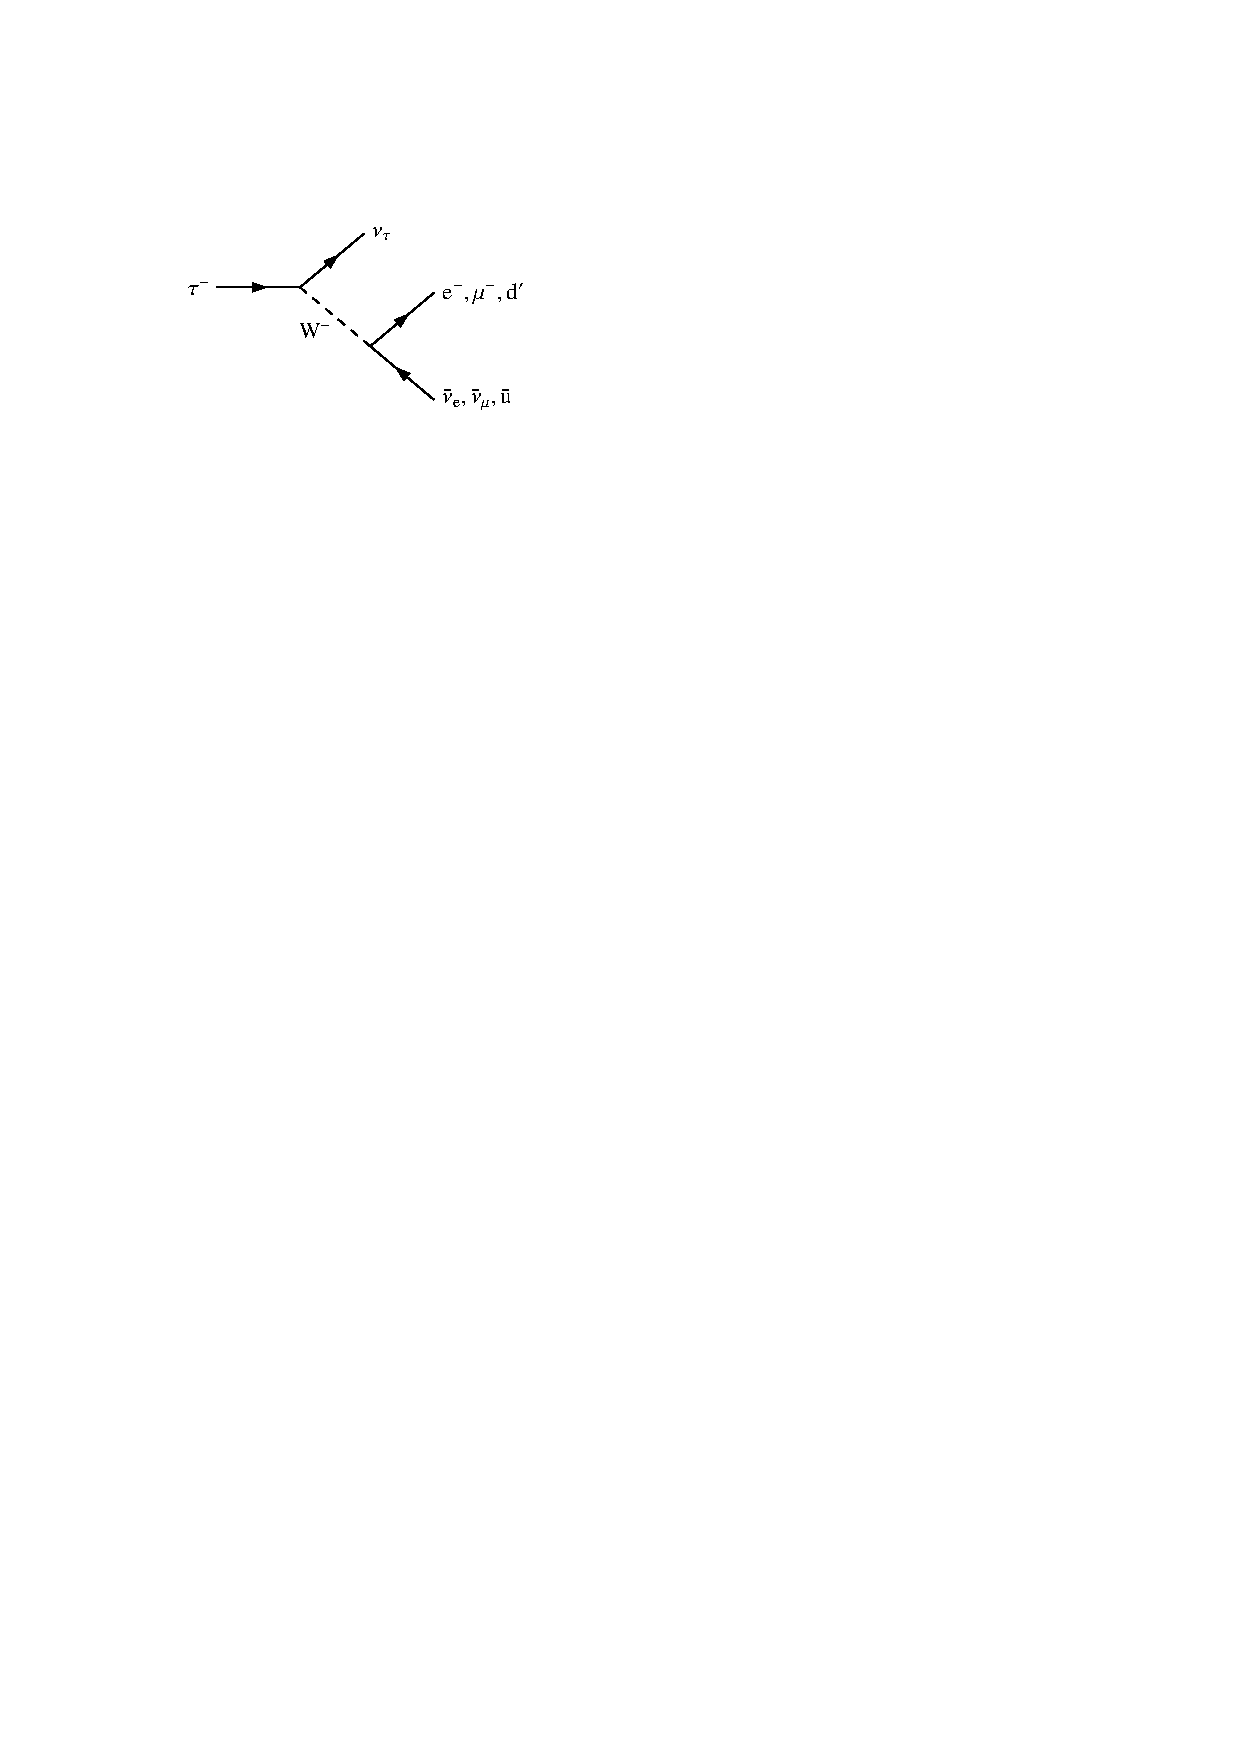
\includegraphics{./figures/theory/tau_decay_feynman.pdf}
    \vspace*{3em}
    \caption{Feynman diagram of the tau decay via the weak interaction. The
      $d^\prime$ is the weak eigenstate mixing the mass eigenstates of the $d$-
      and $s$-quark.}
    \label{fig:tau_feynman}
  \end{subfigure}\hfill
  \begin{subfigure}[b]{0.47\textwidth}
    \centering
    \begin{overpic}[scale=0.9]{./figures/theory/tau_branching_pie_chart.pdf}
      \put (31, 83) {$\pi^- \nu_\tau$}
      \put (-5, 45) {$\pi^- \pi^0 \nu_\tau$}
      \put (16, 7) {$\pi^- 2 \pi^0 \nu_\tau$}
      \put (40.5, 2) {$2 \pi^- \pi^+ \nu_\tau$}
      \put (65, 6.5) {$2 \pi^- \pi^+ \pi^0 \nu_\tau$}
      \put (76.5, 15.5) {other}
      \put (70, 77.5) {$e^- \bar{\nu}_e \nu_\tau$}
      \put (88.5, 41.5) {$\mu^- \bar{\nu}_\mu \nu_\tau$}
    \end{overpic}
    \caption{Tau lepton branching ratios~\cite{pdg}. The mode percentage is
      given with respect to all leptonic (hadronic) modes. Adapted from
      Ref.~\cite{ikai_trigger}.}
    \label{fig:tau_branching_ratios}
  \end{subfigure}
  \caption{Decay and branching ratios of the tau lepton. Charge-conjugate decay
    modes are omitted.}
\end{figure}

The following focuses on hadronic decays and their detector signature. Due to
the short lifetime of the tau lepton, a tau lepton with a momentum of
\SI{20}{\GeV} has a mean decay length of~$\mathcal{O}(\SI{1}{\milli\metre})$.
Therefore, it typically decays before entering tracking systems of particle
detectors. As a result the tau lepton is not observed directly but its decay
products. The boost of tau leptons produced in collider experiments results in
highly collimated decay products. The charged pions and kaons produced in the
decay are considered stable over typical length scales of general-purpose
detectors at hadron colliders. They create hits in the tracking system and
deposit most their energy in the hadronic calorimeters. In contrast to this, the
neutral pions decay almost immediately via the electromagnetic interaction in
the process~\mbox{$\pi^0 \to \gamma\gamma$} with a branching ratio of~\SI{98.823
  +- 0.034}{\percent}~\cite{pdg}. The two photons, which are also highly
collimated, deposit their energy in the electromagnetic calorimeter without
leaving a track in the tracking system. The tau neutrino is not observed
directly and can only be inferred from missing transverse energy in the event.
As a result one defines the visible part of hadronic tau decays as \tauhadvis
and the decay including the neutrino as \tauhad.

\subsection{Identification of Hadronic Tau Decays}
\label{sec:features_tau_decay}

The signature of hadronic tau decays consisting of multiple charged and neutral
hadrons is similar to that of quark- and gluon-initiated jets. The production
cross section of dijet events at the LHC, consisting of two back-to-back jets in
the transverse plane, is multiple orders of magnitude larger than electroweak
processes of interest. Due to the similarity of hadronic tau decays and jets
originating from quarks or gluons, dijet events represent a significant
background in many analyses with hadronically decaying tau leptons in the final
state. Other processes, e.g.\ the production of jets in association with vector
bosons, exist, producing jets that can be falsely reconstructed as hadronic tau
decays.

An identification procedure is required to reduce backgrounds from quark and
gluon jets that are reconstructed as hadronic tau decays. Tau identification
algorithms are able to exploit the differences between hadronic tau decays and
jets. A full identification of hadronic tau decays also requires to discriminate
against electrons and muons faking hadronic tau decays. However, compared to
fake \tauhad from quark- and gluon-jets, this plays a secondary role in the
identification and is not considered here.

In the following the main differences of hadronically decaying tau leptons and
quark- and gluon-initiated jets are summarised:
\begin{description}
\item[Hadron multiplicity] Typically hadronic tau lepton decays consist of one
  or three charged-particle tracks and photons originating from decays of up to
  two neutral pions. In contrast to this, jets from quark and gluons have a
  large average hadron multiplicity~\cite{ellis_stirling_webber}. Therefore, a
  significant discrimination can already be obtained by requiring one or three
  charged-particle tracks in a reconstructed hadronic tau decay.

\item[Isolation] The secondary particles produced in a hadronic tau decay form a
  narrow and collimated jet, which is isolated from other particles in the
  event. The angular distribution of hadrons produced in jets originating from
  quarks and gluons are on average broader than in hadronic tau decays. As a
  result, the signature of hadronic tau decays can be exploited by requiring
  collimated charged-particle tracks in the tracking system and narrow showers
  in the calorimeters.

\item[Decay length] While the short lifetime of tau leptons typically causes
  them to decay before entering the active detector volume, the excellent impact
  parameter resolution and vertexing of recent tracking detectors allows to
  measure deviances of the tau decay vertex from the primary vertex of the
  interaction. In contrast to this, charged-particle tracks in quark- and
  gluon-initiated jets are expected to originate from the primary vertex. This
  can be exploited by measuring deviations of the track impact parameters from
  the primary vertex or by explicitly reconstructing the secondary vertex.

\item[Invariant mass] The invariant mass of the secondary particles produced in
  hadronic tau decays can be used to discriminate against quark and gluon-jets.
  The invariant mass is given by the mass of the tau lepton for tau decays,
  while the mass in unbounded for jets originating from quarks or gluons. When
  partially reconstructing the invariant mass of the secondaries in a tau decay,
  the mass is bounded by the tau lepton mass, thus allowing to distinguish them
  from quark and gluon-jets with larger invariant masses.

\end{description}
Another discriminating feature is the missing transverse energy due to the tau
neutrino created in the decay. For a general purpose tau identification
algorithm this is not used to be largely independent of the remainder of the
event. On average gluon-initiated jets exhibit larger multiplicities and are
broader than jets originating from quarks \cite{ellis_stirling_webber}.
Therefore, the performance of tau identification algorithms strongly depends on
the parton that initiated a jet.

The ATLAS and CMS experiments at the LHC use multivariate analysis techniques
employing variables sensitive to the differences between quark- and
gluon-initiated jets and hadronic tau decays for
identification~\cite{atlas:taurec:run2, cms_tauid}.

\subsection{Tau Lepton Physics at the LHC}

The tau lepton is an important probe of physics at high energy scales, such as
Higgs physics and physics beyond the Standard Model. Hadronic decays make up
approximately two-thirds of the total branching ratio of tau decays and
represent a major contribution to final states involving tau leptons. In the
following the importance of hadronic tau lepton decays for the physics programme
at the LHC is motivated.

\subsubsection{Measurements of the Standard Model Higgs Boson in the
  $\tauhad\tauhad$ Channel}

To investigate the Higgs mechanism of the Standard Model it is important to
measure the Yukawa coupling of the Higgs boson to fermions and show that the
coupling strength is proportional to the mass of the fermion. Due to the
branching ratios of the Standard Model Higgs boson with a mass of about
\SI{125}{\GeV}, the decay modes~$h \to b \bar{b}$ and~$h \to \tau \tau$ are the
most promising. At the LHC the measurement of $h \to b\bar{b}$ is difficult due
to the large background from multijet production, therefore requiring associated
production of the Higgs with a vector boson to limit the background
contribution~\cite{higgs_bb}. This reduces the signal yield due to the smaller
cross section of associated production of the Higgs boson compared to gluon
fusion.

The $h \to \tau\tau$ decay mode offers a promising alternative to measure the
fermionic coupling. In the $h\tau\tau$ coupling measurement of the ATLAS
experiment~\cite{higgs_tautau}, the analysis is split into three
channels~$\taulep\taulep$, $\taulep\tauhad$ and~$\tauhad\tauhad$, depending on
whether the taus decay leptonically or hadronically. Due to the branching
fraction of the tau lepton, the~$\tauhad\tauhad$ channel comprises of more than
\SI{40}{\percent} of~$h \to \tau\tau$ decays, which is only marginally exceeded
by the~$\taulep\tauhad$ channel. The~\tauhad are susceptible to being faked by
jets originating from quark- or gluon-jets. As a result, a performant tau
identification algorithm is required to reduce the background contributions in
the $\tauhad\tauhad$ channel due to multijet production, $W{+}\text{jets}$ and
$t\bar{t}$.

An important discriminating variable used in the~$h \to \tau\tau$
analysis~\cite{higgs_tautau}, partially separating the signal from the
irreducible~$Z / \gamma^* \to \tau\tau$ background is the ditau invariant mass,
$m_{\tau\tau}$. Due to the presence of two neutrinos in final states of the
$\tauhad\tauhad$ channel, the invariant mass cannot be reconstructed
unambiguously. A missing mass calculator (MMC) uses constrains from the
invariant mass of the visible decay products of both tau leptons and the
measured missing transverse momentum to improve the accuracy of the
reconstructed ditau invariant mass~\cite{mmc}. In Figure~\ref{fig:mtautau_mmc}
the reconstructed ditau invariant mass, $m_{\tau\tau}^\text{MMC}$, is depicted
for Higgs bosons produced in the vector boson fusion (VBF) process. Although the
analysis requires two identified tau leptons with additional isolation cuts, a
significant background from fake \tauhad originating from quark- and gluon-jets
is present. As the expected signal contribution of the Higgs boson is smaller
than the background from fake \tauhad, an improvement in the tau identification
algorithm could lead to a higher signal significance in this measurement.

In addition to measuring the $h\tau\tau$ Yukawa coupling,
the~$h \to \tauhad\tauhad$ channel is promising to determine the \cp nature of
the Higgs boson. Assuming a pseudoscalar admixture to the scalar~$h\tau\tau$
coupling, \cp violation would be observed in the $h \to \tau\tau$ decay. A
measurement of \cp violation in the Higgs sector could indicate new physics and
explain the observed matter--antimatter asymmetry in the Universe. The size of
the pseudoscalar admixture is directly encoded in the polarisation of the tau
leptons created in the decay, which can be measured in the angular distributions
of the charged and neutral decay products of the hadronic tau decay including
the neutrino~\cite{harnik, Berge2014}. Inferring the tau polarisation requires a
well-performing tau reconstruction including classifying the decay mode and
reconstructing individual decay products.

\subsubsection{Search for Additional Heavy Neutral Higgs Bosons}

The minimal extension of the Standard Model to include Supersymmetry is called
the Minimal Supersymmetric Standard Model (MSSM). It it introduces an additional
Higgs doublet leading to an extended Higgs sector with two \cp-even neutral
Higgs bosons~$h$ and $H$, a \cp-odd~$A$ boson and two charged~$H^\pm$
bosons~\cite{susy}. The heavy neutral Higgs bosons~$H$ and~$A$ couple preferably
to down-type fermions (i.e.\ fermions with weak isospin~$T_3 = -1/2$), if the
ratio of vacuum expectation values of both Higgs doublets, $\tan\beta$, is
large~\cite{susy}. Therefore, the~$H / A \to \tauhad\tauhad$ channel is
promising to search for additional neutral Higgs bosons.

\begin{figure}[htb]
  \begin{subfigure}[t]{0.48\textwidth}
    \centering
    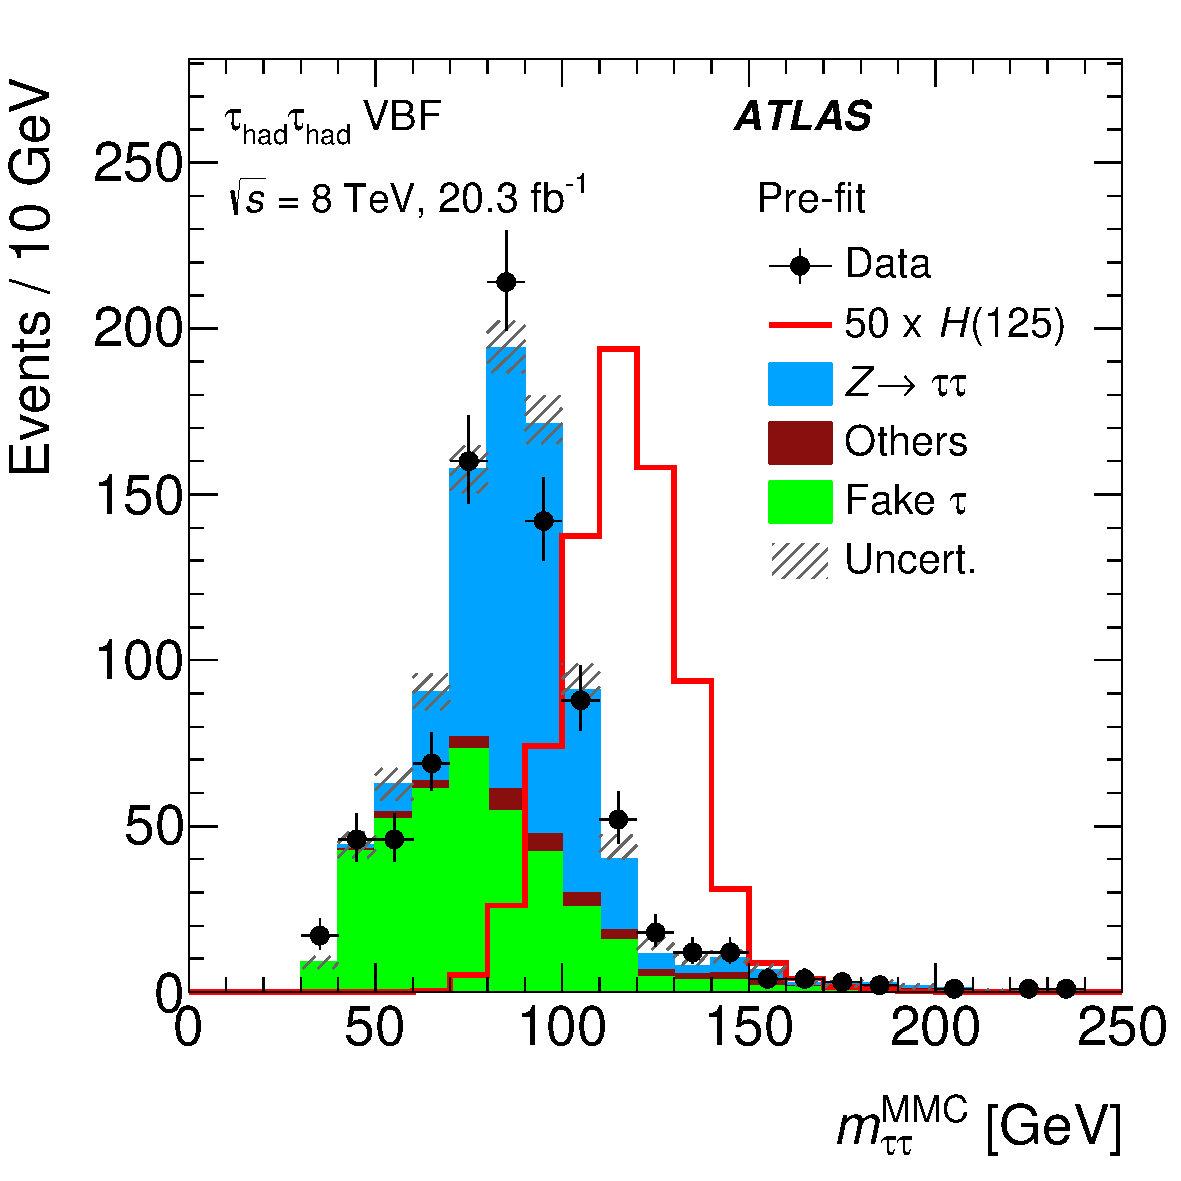
\includegraphics[width=0.98\textwidth]{./figures/theory/htautau_mass_2.pdf}
    \subcaption{Invariant mass of the ditau system reconstructed with the
      missing mass calculator in the~\mbox{$h \to \tauhad\tauhad$} VBF channel
      of the ATLAS $h\tau\tau$ coupling measurement~\cite{higgs_tautau}. The
      scaled contribution of the Standard Model Higgs boson is superimposed.}
    \label{fig:mtautau_mmc}
  \end{subfigure}\hfill
  \begin{subfigure}[t]{0.48\textwidth}
    \centering
    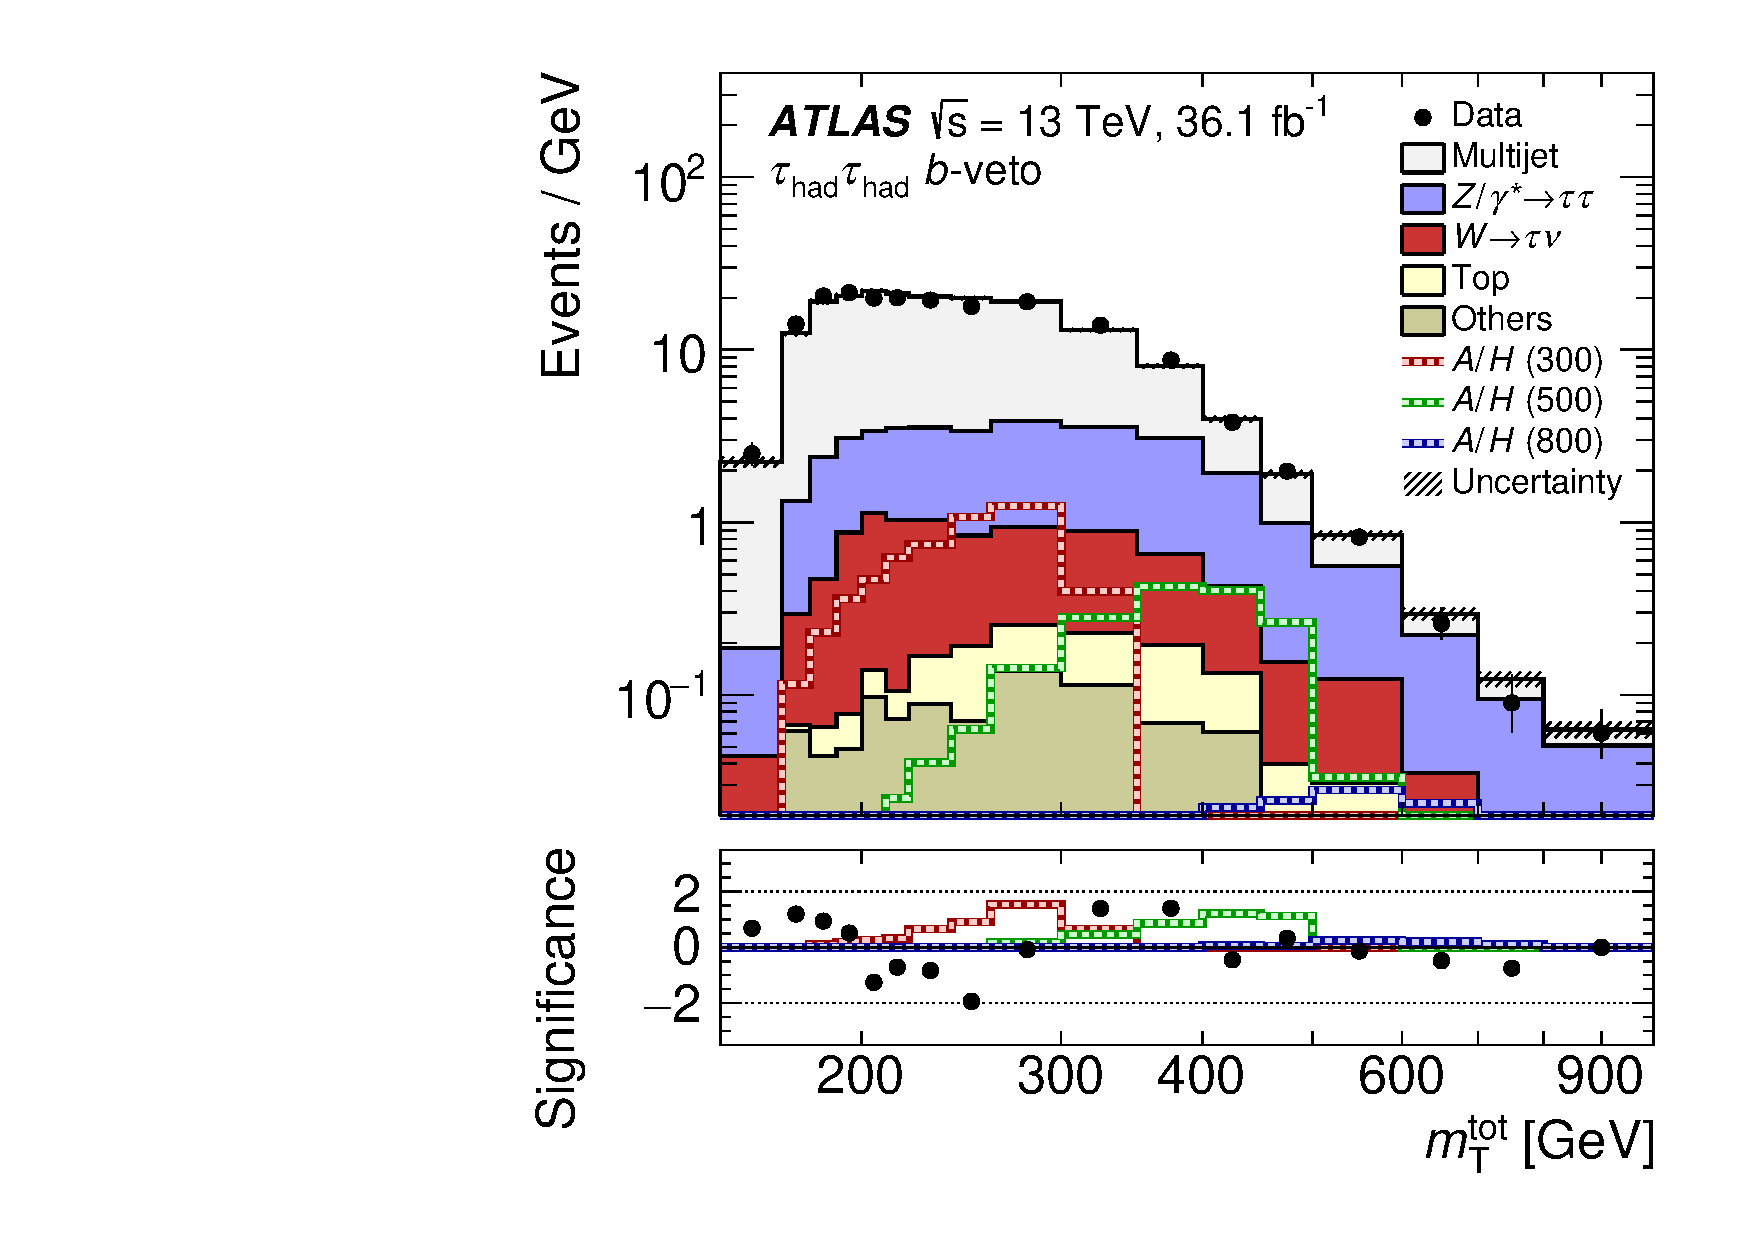
\includegraphics[width=1.0\textwidth]{./figures/theory/zprime_mttot.pdf}
    \subcaption{$m_\text{T}^\text{tot}$ distribution in the $b$-veto category of
      the $\tauhad\tauhad$ channel in the ATLAS search for additional neutral
      Higgs bosons~\cite{zprime}. The signal contribution of $A$ and $H$ bosons
      with different masses and~$\tan\beta = 15$ in the hMSSM model~\cite{hmssm}
      is superimposed.}
    \label{fig:mttot_mssm}
  \end{subfigure}
  \caption{Examples for the use of hadronic tau lepton decays in collider
    experiments at the LHC.}
\end{figure}

To separate signal and background contribution in the ATLAS search for heavy
neutral Higgs bosons~\cite{zprime} the total transverse mass,
$m_\text{T}^\text{tot}$, is used. It is defined as
\begin{align*}
  m_\text{T}^\text{tot} = \sqrt{\left(p_\text{T}^{\tau_1} + p_\text{T}^{\tau_2} + E_\text{T}^\text{miss}\right)^2 - \left(\bm{p}_\text{T}^{\tau_1} + \bm{p}_\text{T}^{\tau_2} + \bm{E}_\text{T}^\text{miss}\right)^2}\eqcomma
\end{align*}
where~$\bm{p}_\text{T}^{\tau_1}$ and~$\bm{p}_\text{T}^{\tau_2}$ are the visible
transverse momenta of the tau leptons and~$\bm{E}_\text{T}^\text{miss}$ the
missing transverse momentum in the event. In Figure~\ref{fig:mttot_mssm} the
$m_\text{T}^\text{tot}$ distribution in the $\tauhad\tauhad$ channel without
associated-production of $b$-quarks is shown. Similar to the~$h\tau\tau$
coupling analysis, the hadronically decaying tau leptons are required to be
identified. Nevertheless, one of the major backgrounds in this analysis are
fake~$\tauhad$ originating from quark- and gluon-initiated jets in multijet
events. Improvements in the tau identification algorithm to further reduce the
multijet background could lead to more stringent mass limits on additional
neutral Higgs bosons.

\subsubsection{Other Areas of Research Interest}

The two examples for analyses involving hadronic tau lepton decays are only a
small part of the tau physics programme at the LHC. An incomprehensive list of
further areas of interest is given in the following:
\begin{itemize}
\item Performance measurements of reconstruction algorithms for hadronic tau
  decays using tag-and-probe in~$Z \to \tau\tau$. Additionally, the
  major~$Z \to \tauhad\tauhad$ background present in many analysis, e.g.\ the
  $h\tau\tau$ coupling analysis or MSSM neutral Higgs boson searches presented
  previously, can be measured.

\item Polarisation measurements of~$Z \to \tau\tau$ and~$h \to \tau\tau$ by
  using the tau decay as a spin-analyser. The tau polarisation could be
  exploited to reduce the~$Z \to \tau\tau$ background in measurements and
  searches of neutral spin-0 resonances in the ditau channel.

\item Theoretical models extending the Standard Model with additional heavy
  gauge bosons~$W^\prime$ and $Z^\prime$ exist that couple preferably to
  fermions of the third generation~\cite{NUGIM, zprimephysics} leading to an
  enhanced production of tau leptons.

\item In addition to searches of additional bosons in the Higgs sector of the
  MSSM, Supersymmetry can be probed via the direct production of other
  supersymmetric particles. An example is the strong production of the
  superpartners of quarks and gluons, the squarks and
  gluinos~\cite{squarks_gluinos}. In the R-parity conserving MSSM model, squarks
  and gluinos are produced in pairs and decay via cascades of Standard Model
  particles until the stable and lightest supersymmetric particle is
  produced~\cite{susy_pheno}. Certain models lead to an enhanced production of
  tau leptons in the decay cascade, making tau leptons an important probe to
  constrain the allowed parameter space of Supersymmetry models.
\end{itemize}

%%% Local Variables:
%%% mode: latex
%%% TeX-master: "mythesis"
%%% End:
